\documentclass{article}
\usepackage[utf8]{inputenc}
\usepackage{amsmath}
\usepackage{amssymb}
\usepackage{graphicx}
\usepackage[document]{ragged2e}

\title{Term Project in CEERI: 

Machine Learning for Structural Health Monitoring}

\author{Abhijay Kemkar \hspace{40} Gitansh Pujari}
\date{\hspace{5}2018A4PS0519P \hspace{35} 2018A3PS0352P}

\setlength{\parskip}{1em}
\setlength{\parindent}{0em}

\begin{document}

\maketitle

\section{Introduction}
\justifying{Structural health monitoring (SHM) is an emerging multidisciplinary field for damage detection and condition monitoring structures. A Survey of technical literature indicates that most of the research efforts on this subject have been in system identification, modal response frequency analysis, and signal processing. Advancements in sensor technologies have enabled economically affordable sensor installations for long-term monitoring of civil engineering structures. With the increasing complexity and heterogeneity of sensor data, data integration and data analysis have become critical issues for decision making concerning the diagnosis of the structural conditions. Sensor-based and nondestructive tests at the local level are necessary for a detailed assessment of the damage. 

Data-driven approaches also establish models for comparison with sensor data, but data-driven models exploit information from previously collected sensor data, referred to as “training data.” A variety of data-driven approaches, particularly machine learning techniques, have been proposed in structural health monitoring (SHM) to assess civil engineering structures. Machine learning in the context of SHM can be described as the task of generating knowledge from past experiences (or, more precisely, from collected sensor data), focusing on the prediction of new sensor data. Machine-learning-based solutions have been employed in several signal processing problems in structural health monitoring, such as solving chaotic dynamic signals.}

\section{Literature Review and Related Works}

\subsection{Application of the Subspace-Based Methods in Health Monitoring of Civil Structures}

\justifying{Subspace-based techniques in the vibration-based damage detection (VDD) of structures assess the health state of designs using vibration parameters, relying on observable variations in modal parameters changes (resonant frequency, damping, and mode shape) or their derivatives as indicators of damage existence. In general, vibration-based methods are primarily applicable for global investigation of structural health and considerable damage that affects modal parameters. Subspace system identification is one of the popular techniques in time-domain to derive modal parameters. Structures in VDD can be broadly classified into mechanical engineering structures and civil engineering structures and the identification methods can be classified into combining input-output measurements and utilizing unknown output measurements.

\begin{center}
    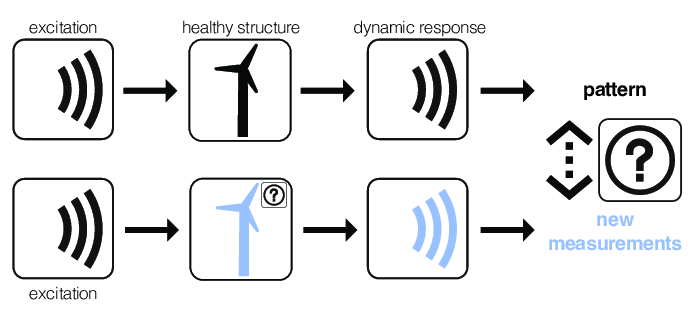
\includegraphics[scale=0.4]{Images/Vibration-based-SHM.png}
    
    \textbf{Figure 1.} Vibration based Damage Detection
\end{center}

The subspace system identification is a more suitable choice for the modal title of closely spaced modal frequencies. Comparison among ERA, and ARMA techniques, subspace system identification has provided the most accurate results. Mathematically, these models are defined as:

\begin{center}
    $x_{k-1} = Ax_k + Bu_k + w_k \ \text{and} \ y_k = Cx_k + Du_k + v_k$
\end{center}

The vectors $u_k \epsilon R^m$ and $y_k \epsilon R^l$ are the observations at time instant k of respectively the m inputs and l outputs of the process. The vector $x_k \epsilon R^n$ is the state vector of the process at discrete time instant k and
contains the numerical values of n states. $v_k \epsilon R^l$ and $w_k \epsilon R^n$ are unobserved vector signals, usually called the measurement process noise.}

\subsubsection{SSI Data Technique}
Data-driven stochastic subspace identification (SSI-DATA) efficacy of three different excitation signals of impact, excellent agreement with estimated modal frequencies of more robust modes. The proposed stochastic subspace (Output-only) method used the Hankel block matrix of the output data to analyze the SSI-DATA. It is not suitable for complex data categories with a large number of sensors, large number of modes of interest, and existing turbulence or no-stationarity. Firstly the Henkel block matrix is constructed from the measured vibration sensor data as

\begin{center}
    $H_{o|2i-1} = \frac{1}{\sqrt{j}}\frac{Y_{o|i-1}}{Y_{i|2i-1}}$
\end{center}

where i and j are the number of rows and columns and Y is the measured data value. Then the QR Decomposition of the matrix H into a product QR of an orthogonal matrix Q and an upper triangular matrix is performed as:

\begin{center}
    $R =\begin{bmatrix}R_{11}&0&0\\R_{21}&R_{22}&0\\R_{31}&R_{32}&R_{33}\\\end{bmatrix} and\ Q = \begin{bmatrix}Q_1^T \\Q_2^T\\Q_3^T\\\end{bmatrix}$
\end{center}

Projection maps/matrices are the vector of response values to the vector of fitted values are defined based in the obtained decomposition as:

\begin{center}
    $P_i = \begin{bmatrix} R_{21}\\ R_{31}\\ \end{bmatrix}Q_1^T, \ P_{i-1} = \begin{bmatrix} R_{31}&R_{32}\\ \end{bmatrix} \begin{bmatrix} Q_1^T\\ Q_2^T\\ \end{bmatrix} \text{where} \ Y_{i|i} = \begin{bmatrix} R_{21}&R_{22} \\ \end{bmatrix} \begin{bmatrix} Q_1^T\\ Q_2^T\\ \end{bmatrix}$
\end{center}

By calculating the Singular value decomposition of the Projection Matrix, which is a factorization of the form UZV, where U is an m×m real unitary matrix, Z is an m×n rectangular diagonal matrix with non-negative real numbers on the diagonal, and V is an n×n real unitary matrix gives:

\begin{center}
    $P_i = U\Sigma V^T$
\end{center}

By factorization of the P matrix, the Kalman filter state sequence $S = O_i^+ P_i$ and observability matrix $O_i = UZ^{1/2}V^T$ can be obtained by the formula $P_i = O_iS_i.O_i^+$ generating the Moore-Penrose pseudo inverse of O. Using similar factorization of the $P_i$ and $S_i$, the one step projection $P_{i-1}$ and Kalman state sequence $S_{i+1}$ can be calculated as:

\begin{center}
    $S_{i+1} = [O_i^+]^+ P_i$
\end{center}

Solving the least squares for the state space matrix A and output matrix C yeilds:

\begin{center}
    $\begin{bmatrix} A\\ C\\ \end{bmatrix} = \begin{bmatrix} S_{i+1}\\ Y_{i|i}\\ \end{bmatrix} S_i^+$
\end{center}

\subsubsection{SSI COV Technique}
SSI-COV Method used hierarchical clustering to identify natural frequencies of each mode of data obtained from the optical sensors. The correlation matrix given below is a table showing correlation coefficients between variables. Each cell in the table shows the correlation between two variables. For our data, it is calculated at i time lags in N number of sensor data where $Y_{i:N-i}$ and $Y_{i:N}$ are the data matrix after removing the last and first i block rows, respectively.

\begin{center}
    $R_i = \frac{1}{N-i}Y_{i:N-i}Y_{i:N}$
\end{center}

The correlation matrix for each sets of time lag is estimated and gathered into $T_{1|i}$ namely block Toeplitz matrix or diagonal-constant matrix. Furthermore the one-lag shifted Toeplitz matrix $T_{2|i+1}$ is also calculated. Then, the estimated correlation is decomposed into orthogonal matrices U and V together with using SVD again as the SSI Data approach as:

\begin{center}
    $T_{1|i} = U_i\Sigma_i V_1^T$
\end{center}

The state matrix is obtained by multiplication of the Observability matrix which is a measure of how well internal states of a system can be inferred from knowledge of its external outputs with the reversed controllability matrix as:

\begin{center}
    $O_i = \begin{bmatrix} C&CA&...&CA^{I-1}\\ \end{bmatrix} \ \text{and} \ \Gamma_i = \begin{bmatrix} A^{i-1}G&...&AG&G\\ \end{bmatrix}$ \\as $T_{1|i} = O_i\Gamma_i$
\end{center}

By splitting the $T_{1|i}$ matrix using identity matrix yields:

\begin{center}
    $O_i = U_1\Sigma_1^{1/2}I^T$ \ and \ $\Gamma_i = I^{-1}\Sigma_1^{1/2}I\V_1^T$
\end{center}

By factorization of the one-lag shifted Toplitz matrix and solving the state space matrix yields:

\begin{center}
    $A = \Sigma_1^{1/2}U_1TT_{2|i+1}V_1\Sigma_1^{1/2}I_T$
\end{center}

\subsubsection{Comparison between SSI DATA and SSI COV}
Improved efficiency was achieved by adopting a stabilization diagram on identified modal parameters using SSI-COV and SSI-DATA techniques. Reference based generalization (SSI-data/ref, SSI/ref, and CSI/ref) are adopted in the software package along with OMA, LMS Cada-X, LMS International, TestLab for modal analysis. Decentralized SSI-DATA algorithm implemented on Imote2 based WSNs. Particle swarm optimization (PSO) with a sequential Niche technique (SNT) was used for the FE model updating of a pedestrian cable-stayed bridge. Singular spectrum analysis (SSA) was also adopted to smoothen the input signal and yield reliable modal parameters as a prepossessing tool for SSI-COV. Several algorithms are introduced based on classical SSI-COV, SSI-DATA, and the combined method to improve the subspace system's performance. The SSI-DATA and SSI-COV algorithms' obtained results are similar in the case of accuracy, but the computation time SSI-COV is much lower than the SSI-DATA approach.

\subsection{Structural health monitoring of bridges: a model-free ANN-based approach to damage detection}
SHM is divided into model-based and model-free approaches. Simulations of train passages behave normally (one baseline model) and abnormal conditions (two damaged models). Based on previous instants' acceleration values in time, the neural networks in the picture can predict future accelerations. Secondly, each network's acceleration prediction errors are statistically characterized by a Gaussian process that supports the choice of a damage detection threshold and then can point out damage on the bridge.

Optimal sensor placement is a crucial part of any damage detection system for which the K-mean clustering-based data-driven machine learning approach is used.  Pre-existing methods are based on the structure's damaged condition's data availability (also called supervised learning). Artificial neural networks are used as outlier or novelty detection methods that provide a qualitative indication of damage in the structure without prior knowledge of how the system behaves when damaged. 

A ROC curve is plotted, a two-dimensional graph in which the true positive rate is plotted against the false-positive rate for a given threshold as there is a need to calculate the costs related to false negatives, which are the most penalizing. 3D finite element model of a single-track railway bridge was developed using FEM software ABAQUS. Traffic-induced vibration was obtained by simulating 300 passages of a train. The train model was based on the HSLM-A4.

\begin{center}
    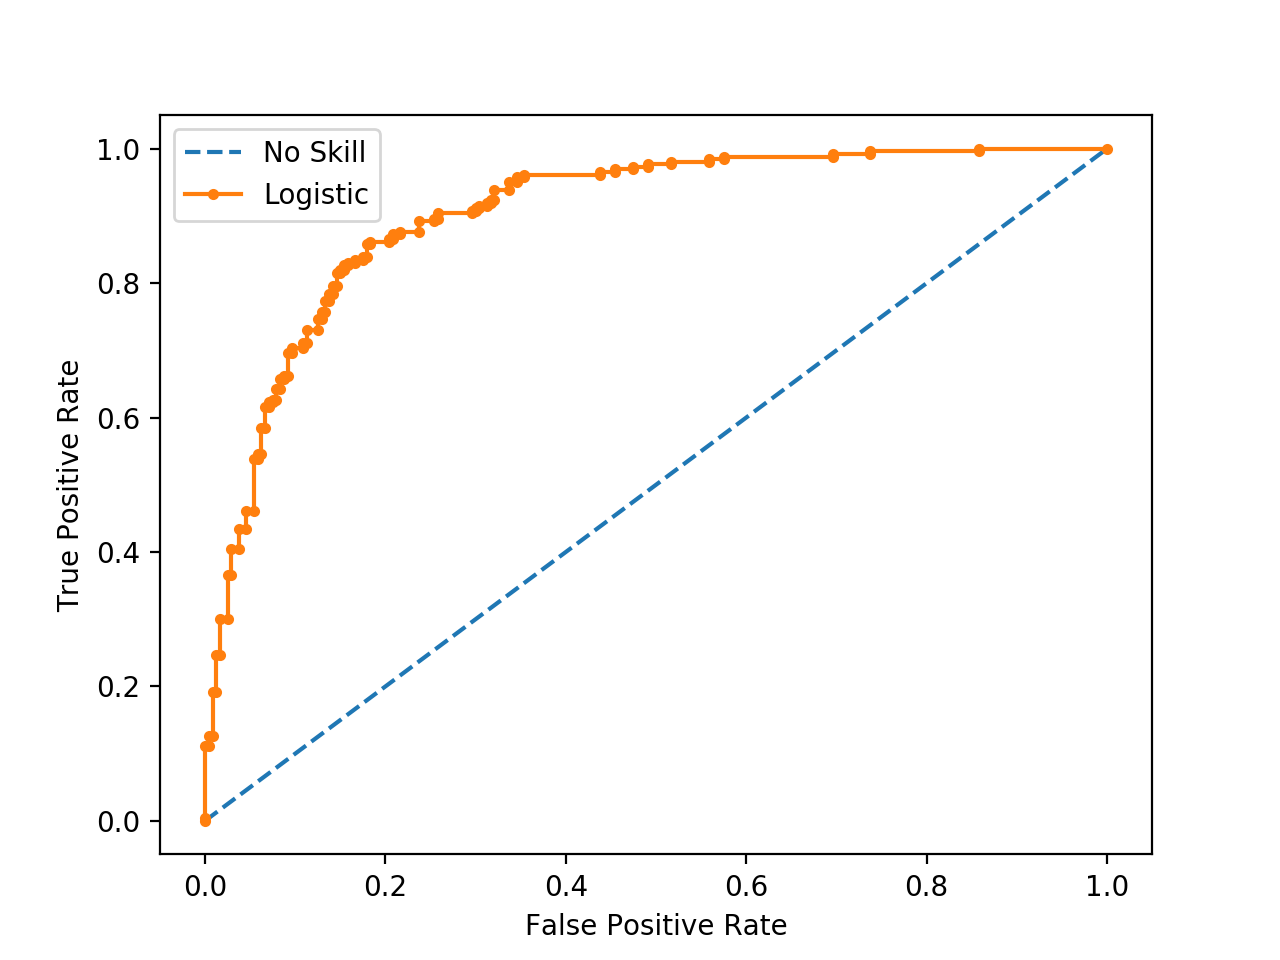
\includegraphics[scale=0.50]{Images/ROC.png}
    
    \text{\textbf{Figure. 2.} Receiver Operating Characteristic Curve plot}
\end{center}

\subsubsection{Working of an Artificial Neural Network}
Each node i is connected to each node j in the previous and following layers over a connection of weight $w_{ij}$. In layer k, a weighted sum is performed at each node i of all the signals from the preceding layer k 1, giving the j excitation of the node; this sum is then passed through a nonlinear activation function f to emerge as the output of the node to the next layer as:

\begin{center}
    $x_i^{(k)} = f(z_i^{(k)}) = f(\sum_{j}^{}w_{ij}^{(k)}x_j^{(k-1)})$
    
    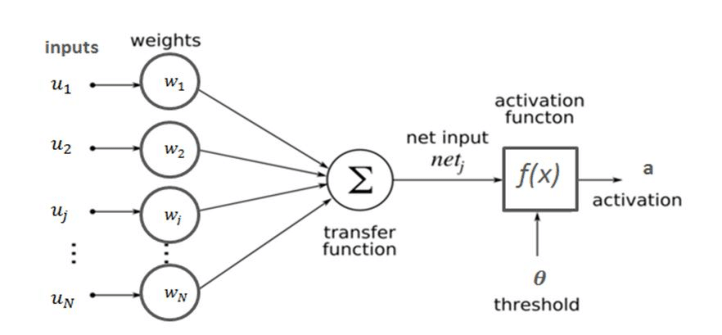
\includegraphics[scale=0.35]{Images/Artificial-Neuron-Structure.png}
    
    \text{\textbf{Figure. 3.} Structure of an Artificial Neural network}
\end{center}

\newpage
150 train passages were used to train the network, and the 150 remaining ones were used for testing and validation of the trained network along with Gaussian white noise with a constant standard deviation of 0.0005 m/$s^2$. Different groups of ANNs trained using Levenburg–Marquardt backpropagation algorithm, with each group having six different networks predicting for one of the six sensors. 49 input neurons representing i accelerations registered by the 6 sensors, the 18 axle loads and 1 axle position relative to a reference point, 30 neurons for the hidden layer, and 1 output neuron representing the current acceleration ant at time t predicted by the sensor n. The ReLU activation funtion was used which is given by:

\begin{center}
    $a=max(0,z)$
    \\
    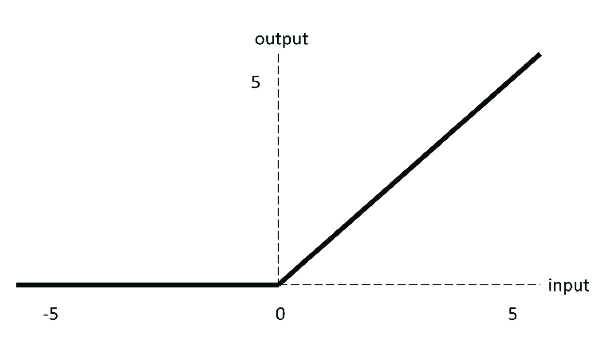
\includegraphics[scale=0.35]{Images/ReLU-activation-function.png}

    \text{\textbf{Figure. 4.} Rectified Linear Unit}
\end{center}

The only problem with the above mentioned model is that the sensors situated closer to the bridge's geometric middle yield a better separation between structural states, while sensors placed near the end supports are not as efficient in this task. Associated predicted errors are normally distributed, the mean and standard deviation of the error is recorded and probability calculation for Bayes Theorem is given by:

\begin{center}
    $P(d|e) = \dfrac{(TP^D \times FN^H) \times p(d)}{(TP^D \times FN^H) \times P(d) + (FP^D TN^H) \times p(h)}$
\end{center}

Regarding future research, once the damage is detected, a subsequent step could be to study the correlation between measurements acquired from the sensing system's different devices, in an attempt to pinpoint the location of the damage. At the same time, optimal sensor placement could be carried out for the system to identify damage in a sufficiently accurate manner while avoiding redundancy in the information.

\subsection{Machine-learning-based approach for post event assessment of damage in a turn-of-the-century building structure}
This study includes support vector machines, neural networks, and Gaussian Naive Bayes techniques for training of the structural health monitoring model. The structural model is trained with the input data as the change in strain magnitudes under known loading configurations. Once the model has been trained, it will be employed to predict the damage for any other loading conditions that the structure was previously never exposed to.  The stiffness equation of the structural system is F = KU where, F is the load matrix, K is the stiffness matrix, and U is the displacement matrix. For the structural components of the building,  damage is defined as the change in their stiffness.
Change in strain due to loads is written as $V= V^d-V^u$ where,

\begin{center}
    $V^d =(\epsilon_{1,d}|\epsilon_{2,d}|......|\epsilon_{n,d}|)^T \ \text{and} \ V^u = (\epsilon_{1,u}|\epsilon_{2,u}|......|\epsilon_{n,u}|)^T $
\end{center}

are strain vectors for damaged and undamaged states, respectively. $\epsilon_{1,d}$ and $\epsilon_{1,u}$ are the strains at location t due to load $F_i$ in damaged and undamaged states, respectively.

In this experiment load tests were performed on selected timber frames, within the building, consisting of girders supported on columns. The load tests involved application of gravity loads, and monitoring of the strains in the girder and column system. Fiber Optic Bragg Grating sensors were employed in the tests.

\begin{center}
    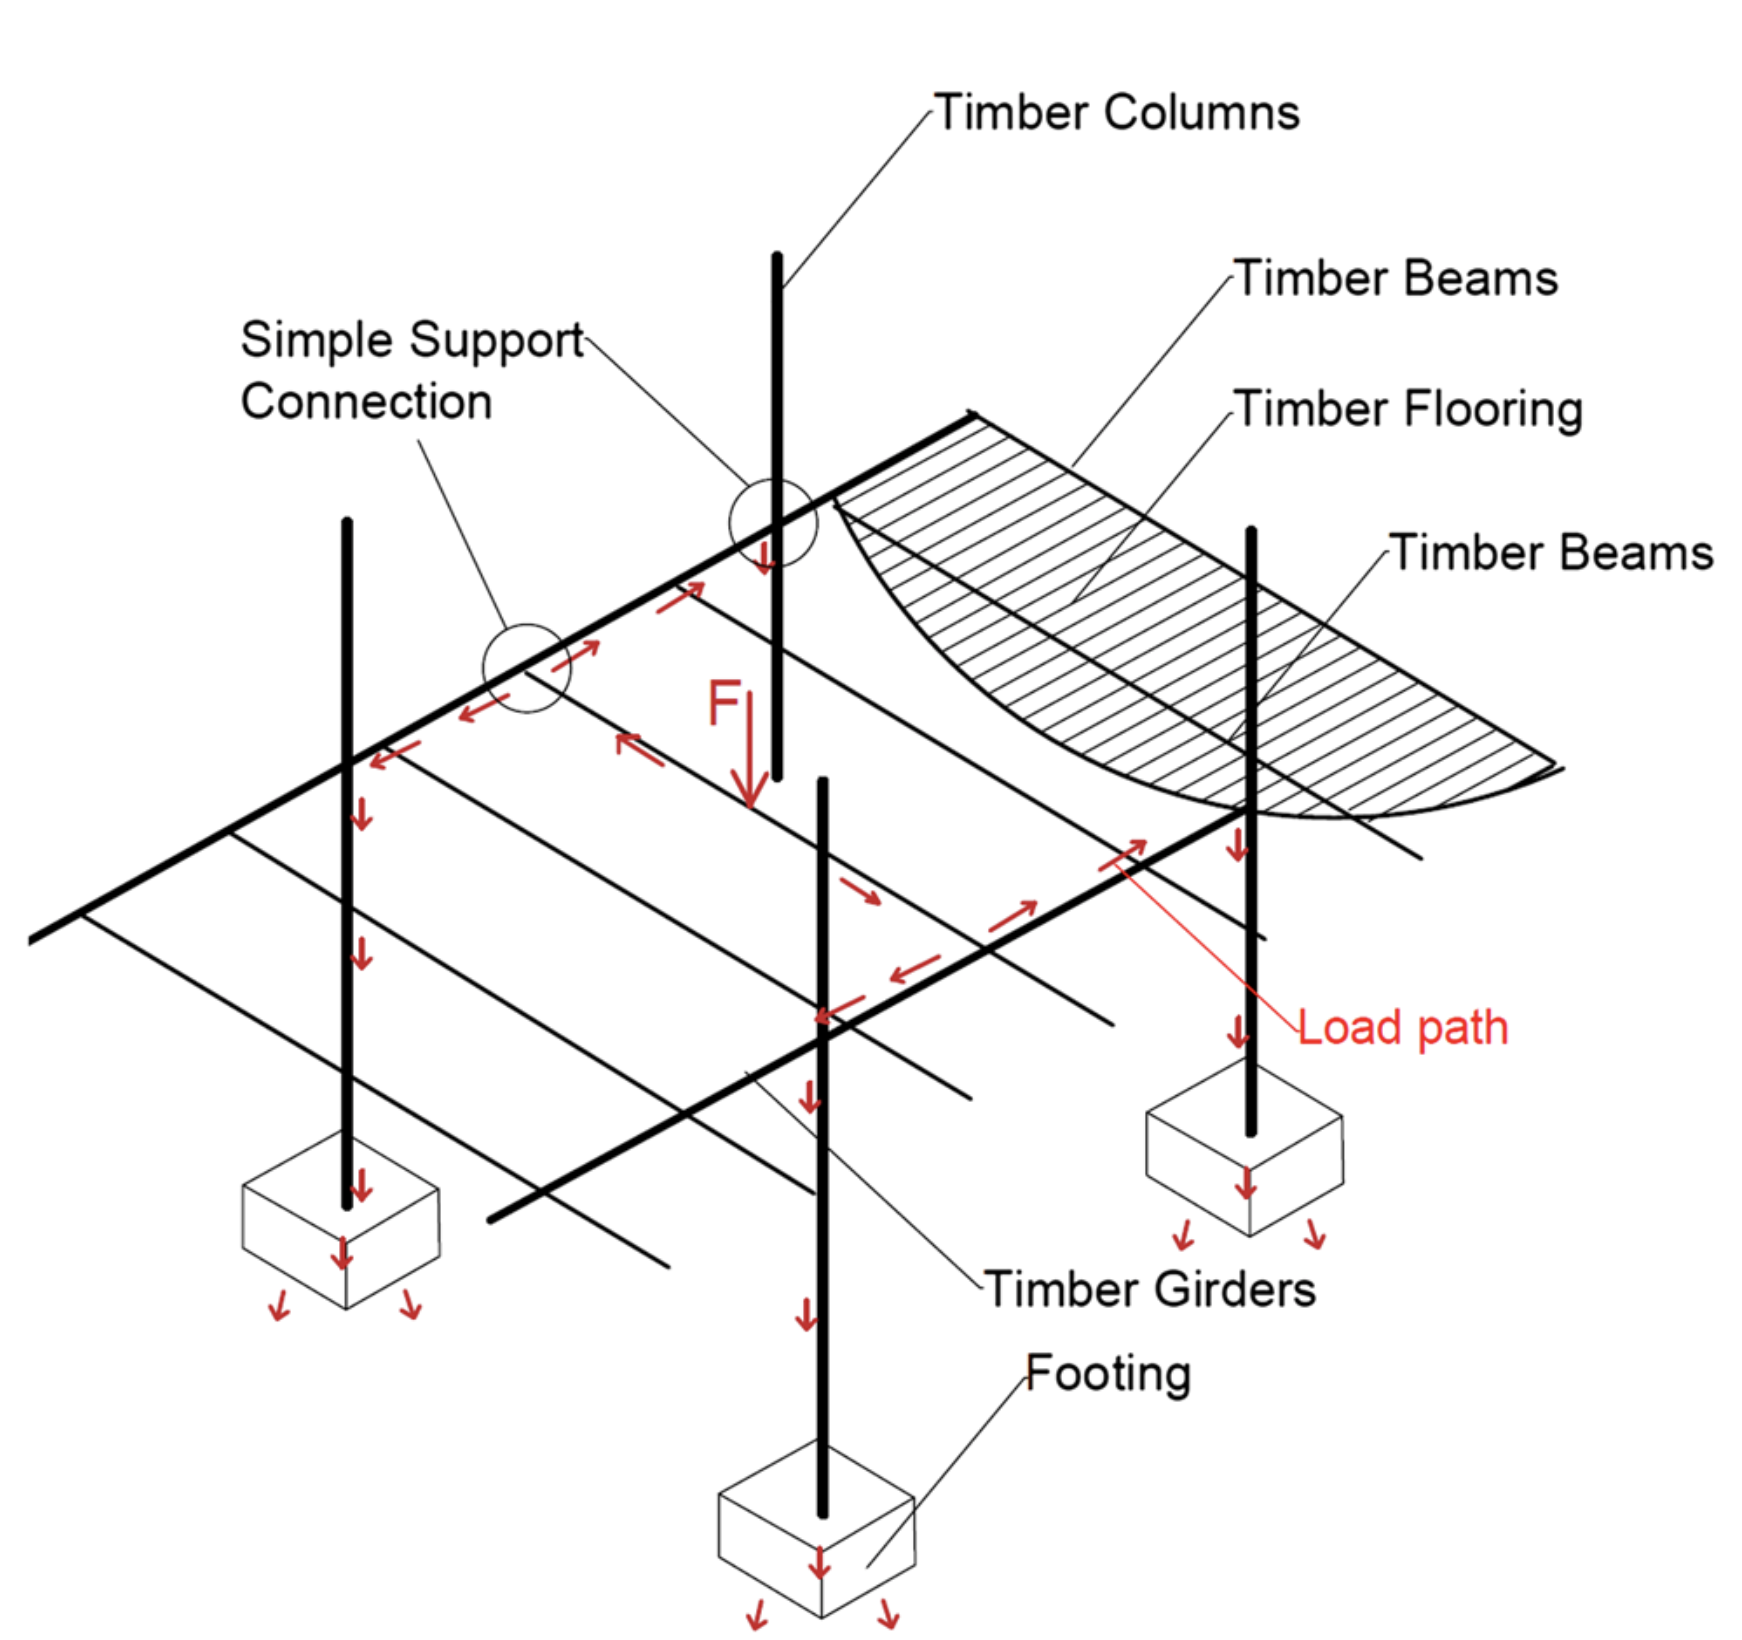
\includegraphics[scale=0.23]{Images/Gravitation_loading.png}

    \text{\textbf{Figure. 5.} Structural system load path}
\end{center}

\justifying
\subsubsection{Experimental Setup}
The thickness of the mortar layer and the FBG sensor are known, the modulus of elasticity of the mortar and brick assembly was obtained. Elongation of the brick and mortar assembly due to the bending strain is equivalent to the elongation of the sensor.

\begin{center}
    $ \epsilon_{m}h_{m}+ \epsilon_{b}(h_{s}-h_{m}) = h_{s}\epsilon_{s}$

    $\text{Where,} \epsilon_{m}=\sigma_{s}/E_{m} \ \text{and} \ \epsilon_{b}=\sigma_{s}/E_{b}$
\end{center}

\justifying
$\epsilon_{m}$ is the strain in the mortar, $\epsilon_{b}$ is the strain in the brick, $h_{m}$ is the thickness of the mortar, $h_{s}$ is the gauge length of the sensor, $\epsilon_{s}$ is strain output of the sensor and $ \sigma_{s}$ is the average stress along the sensor’s gauge length. $h_{m}$ and $h_{s}$ were directly measured. $\sigma_{s}$ was determined by applying the loading pattern that was employed in the finite element model and obtaining the average stress at the location of strain sensor.

\begin{center}
    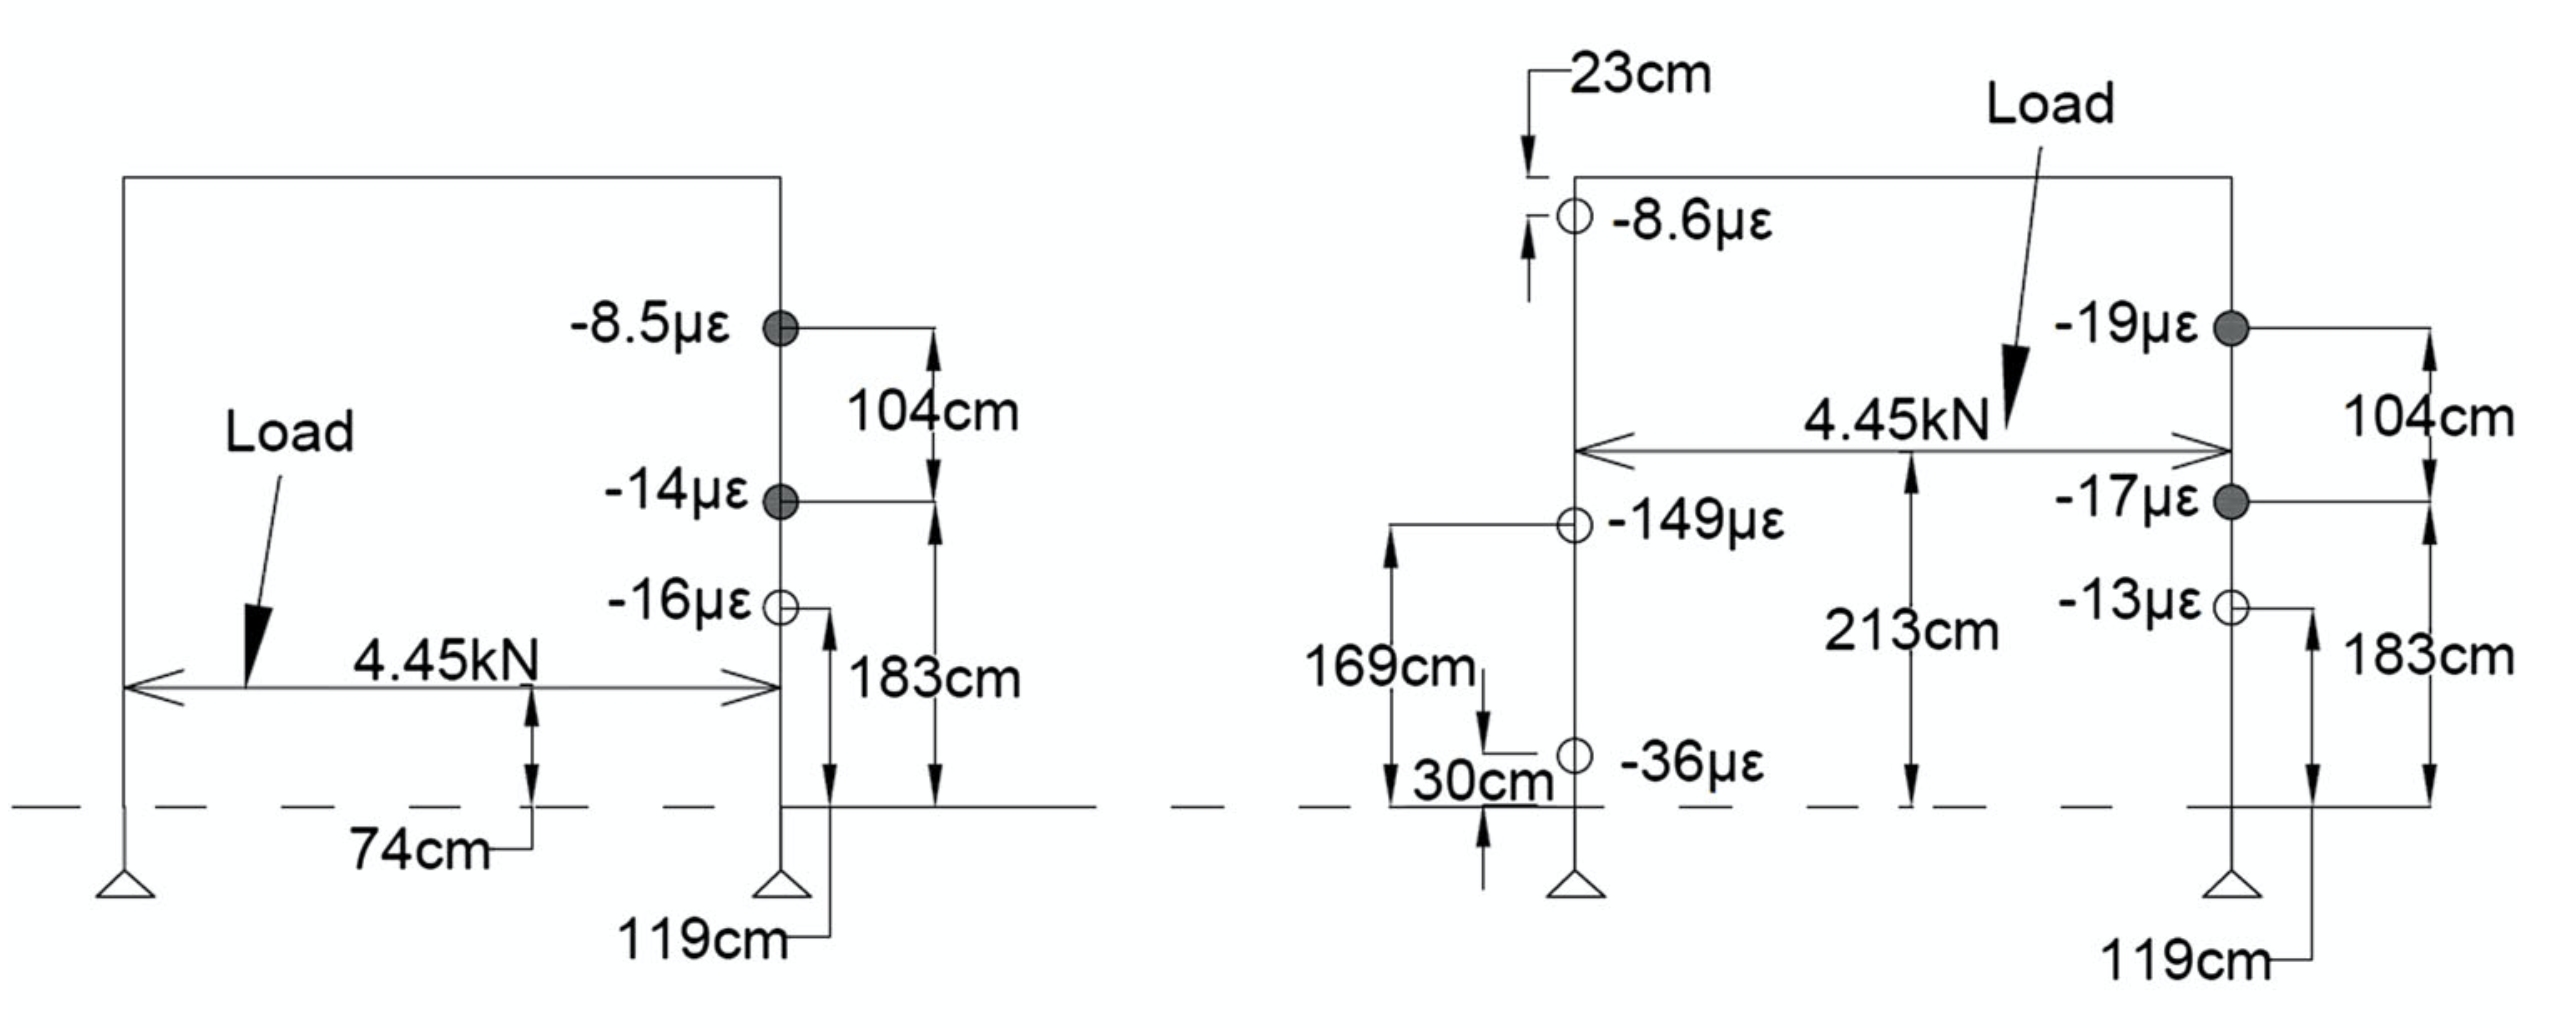
\includegraphics[scale=0.25]{Images/Structural_loading.png}

    \text{\textbf{Figure. 6.} Structural loading: a strain output of frame number}
\end{center}

\subsubsection{Support Vector Machine}
Strain vectors are separated with a maximal margin and Margin is defined as the distance between the closest strain vectors to the hyperplane. Hyper planes separate the strain vectors such that the two sides of a hyperplane, represent two different damage case scenarios.
The hyper plane decision boundary for strain vector, V, can be written as $f(V) = sign((W^T)\phi(V) + b)$ where sign is the signum function, b is the bias and phi is a mapping function. We use f(V) to classify a new data point V .

Maximal margin hyper  plane between the strain vectors is obtained when $W = \sum^n_{i=1} \alpha_{i}y_{i} \phi(V_{i})$ where n is the number of the possible damage cases used in training, y is the binary output which defines the damage case that a strain vector belongs to, and $\alpha_{i}$ are positive coefficients that maximize the following equation:

\begin{center}
    $\sum^n_{i=1}\alpha_{i} - \sum^n_{i,j}\alpha_{i} \alpha_{j}y_{i}y_{j}\phi(V_{i})\phi(V_{j}) \ \text{such that} \ \sum^n_{i=1}\alpha_{i}y_{i} = 0$

    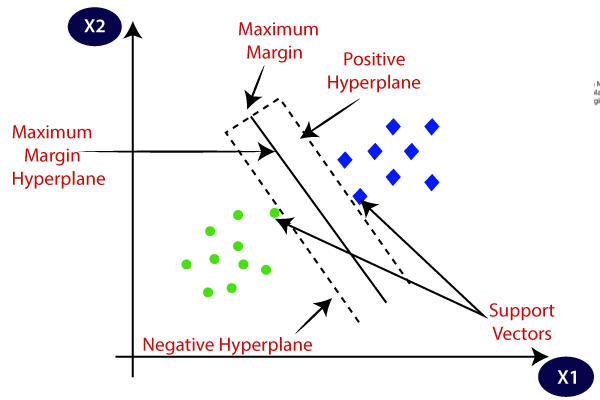
\includegraphics[scale=0.39]{Images/support-vector-machine-algorithm.png}

    \text{\textbf{Figure. 7.} Support Vector Machine Hyperplane}

\end{center}

\subsubsection{Neural Network}
Neural network that we are using is multi-layer feed-forward network which consists of input layer (pertains to strain vector V), hidden layers and output layer (pertains to damage case number). About 100 nodes were used in hidden layer. f1 is the hyperbolic tangent function and f2 is a linear activation function.

\begin{center}
    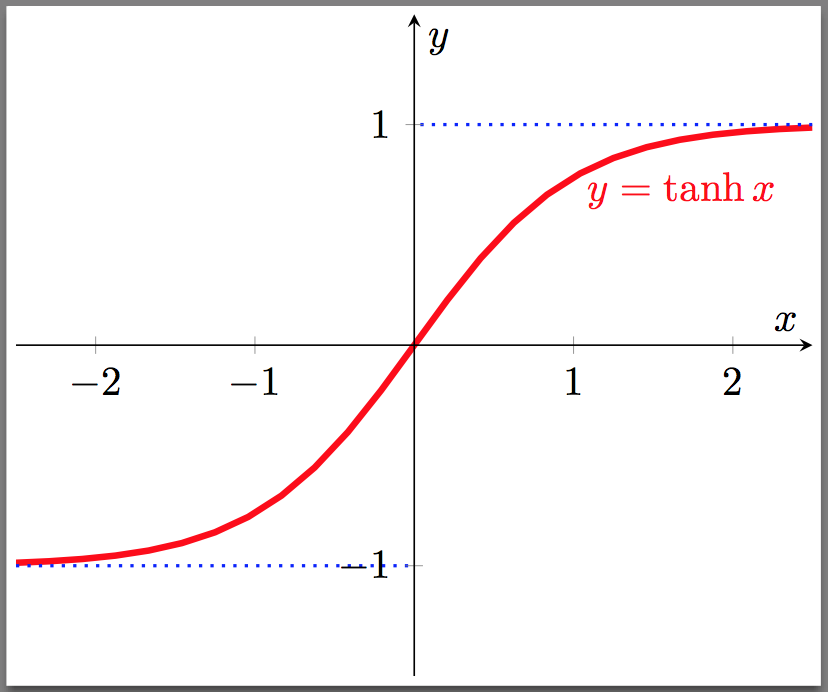
\includegraphics[scale=0.33]{Images/tanh.png}
    
    \text{\textbf{Figure. 8.} hyperbolic tangent function}
    
    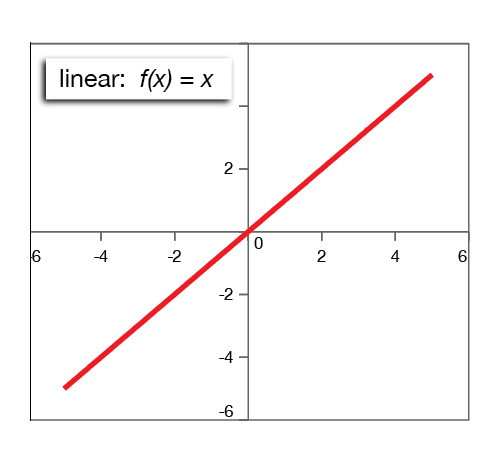
\includegraphics[scale=0.31]{Images/linear.png}
    
    \text{\textbf{Figure. 9.} linear activation function}
\end{center}

The relationship between the layers is then determined by back propagation algorithm and gradient descent to achieve the correct damage case number for a given training input.

\subsubsection{Gaussian Naive Bayes}
Gaussian Naive Bayes (GNB) is a statistical approach based on probabilities and Bayes theorem. It assumes that the predictors, that are considered to be the sensors data in this work, are independent from each other. GNB estimates the probability for all possible damage cases and those cases having the highest probability is then considered to be the predicted damage case. Conditional probability of the damage case $d_i$ for a given set of sensors data can be written as 

\begin{center}
    $P(d_{i}/X) =  P(V/d_{i})P(d_{i})/P(V)$
\end{center}

where V is the strain vector and P() is the probability function. Since the output is independent we can write:

\begin{center}
    $P(V/d_{i}) = Pi_{t} P(v_{t}/d_{i})$
\end{center}

%where $P(v_{t}/d_{i})$ is normally distributed. The predicted damage case, d, is then obtained by $ d = \argmax_{i} P(d_{i}/X) $, where argmax is arguments of maxima which pertains to the damage case, i, that maximizes the function P(d_{i}/X).	

\begin{center}
    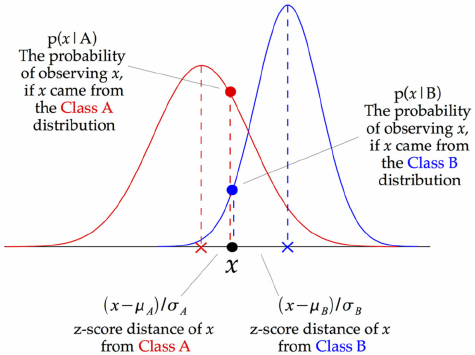
\includegraphics[scale=0.5]{Images/GNB.png}
    
    \text{\textbf{Figure. 10.} Probability distribution of Gaussian Naive Bayes}
\end{center}

\subsection{Machine learning techniques for structural health monitoring}
This paper reports on an embedded machine learning approach for decentralized, autonomous sensor fault detection in wireless sensor networks which is based on the principle of analytical redundancy, which enhances the reliability and accuracy of SHM systems.Instead of physically installing multiple sensors for measuring one single parameter, analytical redundancy takes advantage of the redundant information inherent in the SHM system and utilizes the coherences and relationships between the sensors installed in the structure.
Two general approaches exist for assessing the structural condition are physics-based approaches and data-driven approaches.

Data-driven approaches are particularly useful when 

\indent(i) large quantities of sensor data are available.
\\\indent(ii) the physical characteristics of the structure are complex to model
\\\indent(iii) the computational efforts are to be reduced

data-driven models exploit information from previously collected sensor data, referred to as “training data”. Sensor faults and miscalibrations substantially affect sensor data and may compromise the reliability and accuracy of SHM specifically in data-driven approaches. Machine learning is applied to detect such hidden, non-evident, or inadequately described phenomena.

\begin{center}
    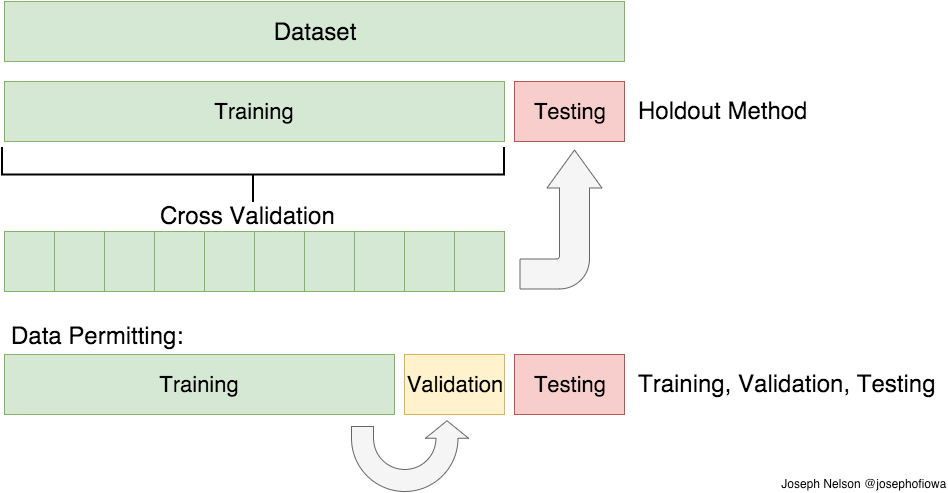
\includegraphics[scale=0.3]{Images/TTV_split.png}
    
    \text{\textbf{Figure. 11.} Train-Test-Validation split}
\end{center}

Machine learning techniques can be classified as:

(i) Supervised learning which provides a learning scheme with “labeled data”, It is used for identifying the type and severity of damage (SVM, naive Bayes classifiers, and feed- forward NN).

\begin{center}
    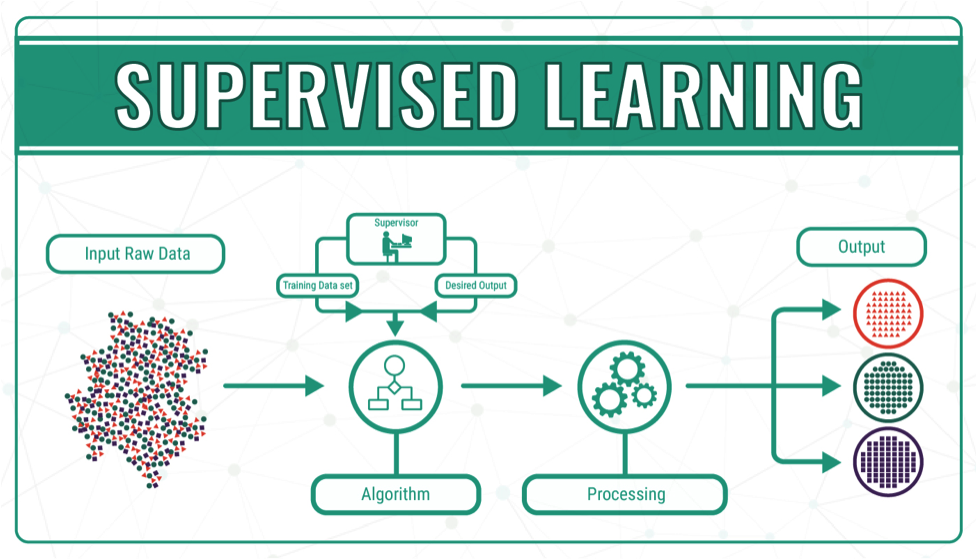
\includegraphics[scale=0.6]{Images/supervised.png}

    \text{\textbf{Figure. 12.} Supervised Learning approach}
\end{center}

(ii)Unsupervised learning encompasses the detection of patterns within the data sets consisting of “unlabeled data”, i.e. data sets with unspecified outputs .It is used for identifying the existence and location of damage (k-means and self-organizing maps).

\begin{center}
    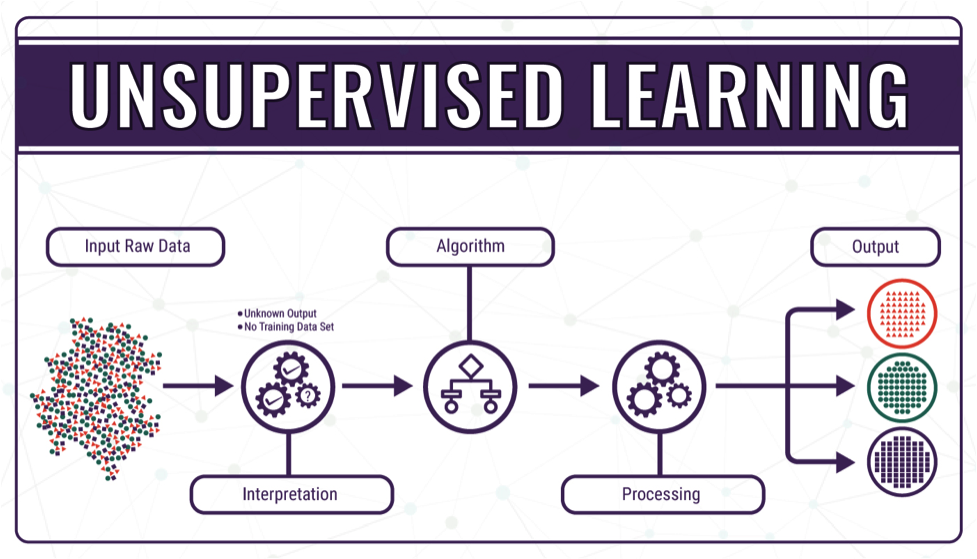
\includegraphics[scale=0.6]{Images/unsupervised.png}

    \text{\textbf{Figure. 13.} Unsupervised Learning approach}
\end{center}

Machine learning  algorithms can be classified as :
(i) logic-based algorithms ,(e.g., decision trees and rule-based classifiers)
(ii) perceptron-based algorithms or neural networks,(e.g., single-layer perceptron, multi-layered perceptron and radial basis function networks)
(iii) statistical learning, (e.g., naive Bayes classifiers and Bayesian networks)			
(iv) instance-based learning (e.g., k-nearest neighbor algorithm)
(v) support vector machines

The peak amplitudes of the frequency spectrum, obtained by the Fourier transformation of acceleration response data are correlated. The correlation can be exploited to predict the modal peak amplitudes of selected sensors, using the modal peak amplitudes of correlated sensors as input data.  Deviations between expected amplitudes and actual amplitudes (i.e. from the measured data) are indicative of sensor faults and miscalibrations. A wireless SHM system is designed that comprises wireless sensor nodes, each of which including an integrated 3-axis accelerometer, a base station, and a host computer.

\begin{center}
    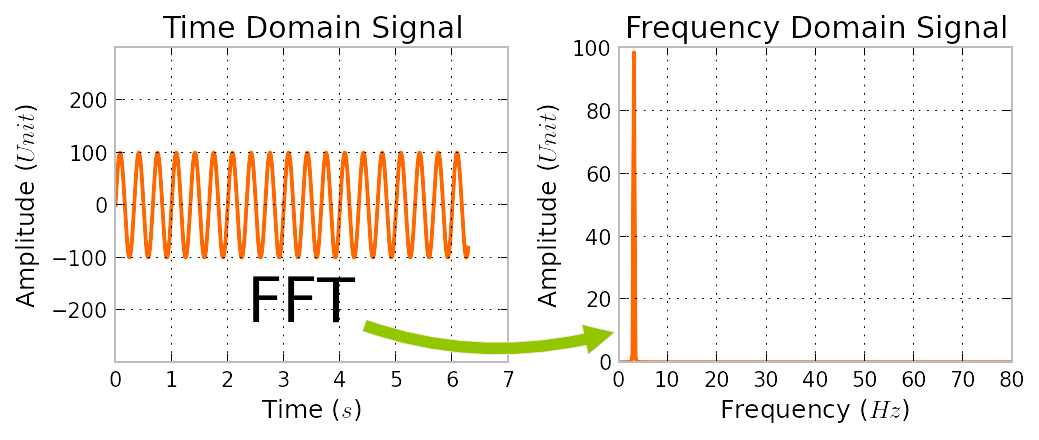
\includegraphics[scale=0.25]{Images/FFT.png}
    
    \text{\textbf{Figure. 14.} Fast Fourier transform on sample data}
\end{center}

The ANNs consist of three layers of neurons: an input layer of k neurons, a hidden layer of m neurons and  an output layer of one neuron. M neurons (hidden layer) are present to account for the nonlinear relationship among the modal peak amplitudes of different sensors whereas the output layer neuron represents the predicted modal peak amplitude of the sensor under consideration. The data is propagated through the ANN via the “synapses” (i.e. connections between neurons), based on the weight of each connection and the accuracy of output is expressed through the RMS error between the expected and the actual amplitudes.

\begin{center}
    $\epsilon_{RMS}=\frac{1}{N}{\sum_{i=1}^{N}\sqrt{{F_{expectedi}(\omega_{1})^{2}-F_{actuali}(\omega_{1})^{2}}}}$
\end{center}

In the equation $\epsilon_{RMS}$ is the root mean squared error, N is the number of testing sets, $F_{expected}$ is the expected modal peak amplitude, $F_{actual}$ is the actual amplitude, and $\omega_{1}$ is the fundamental eigenfrequency. For testing the data set is divided to 80\% training sets to establish the relationship between input and output , 10\% validation sets to decide when to stop training, and 10\% test sets to check the predictive power of the trained ANN.

\section{Implementation}
\subsection{Artificial Neural Network}
\subsubsection{Code Setup}
We started with finding a relevant database for the training and testing of our model. On finding it we first normalised the data-set to make it consistent and then the features were taken as first 12 columns and was stored in X and the label or target was taken as last 2 columns of the dataset and was stored in y. The the the dataset was split into two parts i.e. training and test dataset respectively.

Then we wrote following functions to implement the ANN model :-
\\\textbf{Initialization} :- In this Weights are initialized to random values in the range [0, 0.01) using np.random.rand appropriately and biases are initialized to zero.
\\\textbf{feed\_forward} :- This function computes the output of a full forward pass of the network, using the formulae, z \textbf{=} WX + b and a \textbf{=} g(z)  {g being the non linear function} and then we applied 'forward prop' for each layer according to the architecture defined. 
\\\textbf{regularization\_L2} :- we have used Ridge regularisation as no feature selection was needed to be done.

\subsubsection{Challenges}
Due to non availability of data set the major challenge was to find a relevant data set for our model. Then after training the model we found that it was only 55\% accurate on test data set whereas a 97\% accuracy on the train one. Therefore the next challenge was to find out the reason of this poor value.

\subsubsection{Results}
On training the dataset we get about 55\% accuracy on the test split of the dataset and when the plot is made between loss and no. of iterations it comes to be a negative slop as it needs to be. 

The value of accuracies are:
\\Accuracy on train is :-  0.9302325581395349
\\Accuracy on test is :-  0.5555555555555556

\begin{center}
    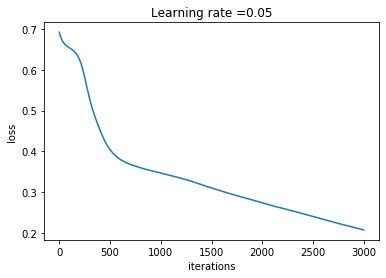
\includegraphics[scale=0.7]{Images/Loss.png}
    
    \text{\textbf{Figure. 14.} Loss graph}
\end{center}

\subsection{Data-driven stochastic subspace identification}
\subsubsection{Code Setup}
The input matrix was assumed to be a random 3 by 3 martix using the rand command in matlab. Then the matrix was converted to a Henkel block matrix which was passed for a QR factorization into an upper triangular matrix R and a matrix Q. The singular value decomposition of the projection of the 2 matrix was carried out which resulted the determination of the observability and shifted observability matrix which in turn were used to calculate the state and output matrix

%\subsubsection{Challenges}


\subsubsection{Results}
The following are the matrices obtained at every step of the SSI-DATA algorithm.

\scriptsize 
$A = \begin{bmatrix}
    0.0975 & 0.9575 & 0.9706 \\
    0.2785 & 0.9649 & 0.9572 \\
    0.5469 & 0.1576 & 0.4854 \\
    \end{bmatrix}$
    
$H = \begin{bmatrix}
    0.0975 & 0.2785 & 0.5469 & 0.9575 & 0.9649 & 0.1576 & 0.9706 & 0.9572 & 0.4854 \\
    0.2785 & 0.5469 & 0.9575 & 0.9649 & 0.1576 & 0.9706 & 0.9572 & 0.4854 & 0 \\
    0.5469 & 0.9575 & 0.9649 & 0.1576 & 0.9706 & 0.9572 & 0.4854 & 0      & 0 \\
    0.9575 & 0.9649 & 0.1576 & 0.9706 & 0.9572 & 0.4854 & 0      & 0      & 0 \\
    0.9649 & 0.1576 & 0.9706 & 0.9572 & 0.4854 & 0      & 0      & 0      & 0 \\
    0.1576 & 0.9706 & 0.9572 & 0.4854 & 0      & 0      & 0      & 0      & 0 \\
    0.9706 & 0.9572 & 0.4854 & 0      & 0      & 0      & 0      & 0      & 0 \\
    0.9572 & 0.4854 & 0      & 0      & 0      & 0      & 0      & 0      & 0 \\
    0.4854 & 0      & 0      & 0      & 0      & 0      & 0      & 0      & 0 \\
    \end{bmatrix}

$Q = \begin{bmatrix}
    -0.0468 & -0.1519 & -0.2543 & -0.4755 &  0.3776 & -0.3542 &  0.6441 &  0.0099 &  0.0322 \\ 
    -0.1335 & -0.2489 & -0.4105 & -0.2442 & -0.4033 &  0.6930 &  0.2094 &  0.0366 & -0.0634 \\ 
    -0.2621 & -0.4020 & -0.1816 &  0.4164 &  0.6754 &  0.2840 & -0.1196 & -0.0920 &  0.0608 \\ 
    -0.4590 & -0.1738 &  0.4364 & -0.6175 &  0.1289 &  0.0778 & -0.3920 &  0.1049 & -0.0034 \\ 
    -0.4625 &  0.4318 & -0.6304 & -0.0511 & -0.0114 & -0.2421 & -0.3361 & -0.0544 & -0.1581 \\ 
    -0.0755 & -0.6333 & -0.1735 &  0.0698 & -0.3977 & -0.4491 & -0.2012 & -0.1649 &  0.3615 \\ 
    -0.4652 & -0.1606 &  0.1852 &  0.3547 & -0.2072 & -0.1880 &  0.2952 &  0.4994 & -0.4276 \\ 
    -0.4588 &  0.1832 &  0.2855 &  0.1314 & -0.1432 &  0.0549 &  0.3391 & -0.7114 &  0.1116 \\ 
    -0.2326 &  0.2763 &  0.0063 &  0.0951 & -0.0112 &  0.0949 &  0.1330 &  0.4398 &  0.8001 \\
    \end{bmatrix}$
    
$R = \begin{bmatrix}
    -2.0863 &       0 &       0 &       0 &       0 &       0 &       0 &       0 &       0 \\ 
    -1.5941 & -1.3424 &       0 &       0 &       0 &       0 &       0 &       0 &       0 \\ 
    -1.2257 & -1.0017 & -1.3266 &       0 &       0 &       0 &       0 &       0 &       0 \\ 
    -1.1397 & -0.5118 & -0.9322 & -1.2396 &       0 &       0 &       0 &       0 &       0 \\ 
    -0.9843 & -0.5328 & -0.3746 & -0.7090 &  1.0742 &       0 &       0 &       0 &       0 \\ 
    -0.6106 & -0.7346 & -0.4005 & -0.2131 &  0.3771 &  0.9263 &       0 &       0 &       0 \\ 
    -0.3004 & -0.5808 & -0.7279 & -0.4931 &  0.3082 &  0.4573 &  0.7675 &       0 &       0 \\ 
    -0.1095 & -0.2662 & -0.4427 & -0.5736 &  0.1656 & -0.0027 &  0.7181 &  0.0272 &       0 \\ 
    -0.0227 & -0.0737 & -0.1234 & -0.2308 &  0.1833 & -0.1719 &  0.3126 &  0.0048 &  0.0156 \\ 
    \end{bmatrix}$
    
$U = \begin{bmatrix}
    -0.3849 &  0.6007 &  0.3864 &  0.0096 & -0.3553 &  0.4165 &  0.2030 & -0.0101 &  0.0252 \\ 
    -0.4382 &  0.3695 & -0.3638 & -0.1685 & -0.1884 & -0.5604 & -0.3952 &  0.0481 & -0.0510 \\ 
    -0.4489 & -0.0428 & -0.4255 &  0.5354 &  0.2448 & -0.0143 &  0.5076 & -0.0971 &  0.0411 \\ 
    -0.4223 & -0.2431 &  0.4216 &  0.3893 &  0.2938 &  0.0907 & -0.5715 &  0.1078 &  0.0219 \\ 
    -0.3520 & -0.1498 &  0.3836 & -0.5412 &  0.3899 & -0.2970 &  0.3827 & -0.0135 & -0.1637 \\ 
    -0.2718 & -0.1516 & -0.3857 & -0.4767 &  0.1604 &  0.5490 & -0.2068 & -0.2373 &  0.3178 \\ 
    -0.2452 & -0.4719 & -0.1401 & -0.0954 & -0.4721 &  0.1705 &  0.0940 &  0.5732 & -0.3149 \\ 
    -0.1410 & -0.3886 &  0.1506 &  0.0641 & -0.5013 & -0.1552 &  0.0036 & -0.7245 & -0.0445 \\ 
    -0.0453 & -0.1502 &  0.1461 & -0.0041 & -0.2004 & -0.2478 &  0.1423 &  0.2580 &  0.8750 \\
    \end{bmatrix}$
    
$S = \begin{bmatrix}
     4.1226 &       0 &       0 &       0 &       0 &       0 &       0 &       0 &       0 \\ 
          0 &  1.9411 &       0 &       0 &       0 &       0 &       0 &       0 &       0 \\ 
          0 &       0 &  1.2832 &       0 &       0 &       0 &       0 &       0 &       0 \\ 
          0 &       0 &       0 &  1.1316 &       0 &       0 &       0 &       0 &       0 \\ 
          0 &       0 &       0 &       0 &  0.8607 &       0 &       0 &       0 &       0 \\ 
          0 &       0 &       0 &       0 &       0 &  0.8159 &       0 &       0 &       0 \\ 
          0 &       0 &       0 &       0 &       0 &       0 &  0.6924 &       0 &       0 \\ 
          0 &       0 &       0 &       0 &       0 &       0 &       0 &  0.0189 &       0 \\ 
          0 &       0 &       0 &       0 &       0 &       0 &       0 &       0 &  0.0140 \\ 
    \end{bmatrix}$
    
$V = \begin{bmatrix}
     0.7606 & -0.5589 & -0.2376 & -0.0052 &  0.1466 & -0.1629 & -0.0674 &  0.0001 & -0.0002 \\ 
     0.4426 &  0.1294 &  0.6299 &  0.1483 & -0.0533 &  0.5340 &  0.2839 & -0.0008 &  0.0007 \\ 
     0.3581 &  0.4813 &  0.1555 & -0.5639 & -0.2540 & -0.2440 & -0.4170 &  0.0019 & -0.0008 \\ 
     0.2531 &  0.4792 & -0.5950 &  0.0123 & -0.1257 &  0.0531 &  0.5776 & -0.0028 &  0.0002 \\ 
    -0.1426 & -0.2346 &  0.2144 & -0.6898 &  0.2487 & -0.1600 &  0.5615 & -0.0018 & -0.0021 \\ 
    -0.0863 & -0.1697 & -0.3482 & -0.4283 & -0.0366 &  0.7715 & -0.2499 & -0.0045 &  0.0058 \\ 
    -0.0736 & -0.3545 &  0.0361 & -0.0251 & -0.9121 & -0.0712 &  0.1722 &  0.0170 & -0.0085 \\ 
    -0.0010 & -0.0058 &  0.0037 &  0.0015 & -0.0170 & -0.0066 &  0.0011 & -0.9769 &  0.2127 \\ 
    -0.0002 & -0.0012 &  0.0018 & -0.0001 & -0.0036 & -0.0047 &  0.0032 &  0.2129 &  0.9771 \\
    \end{bmatrix}$
    
$Oi = \begin{bmatrix}
     2.0304 &       0 &       0 &       0 &       0 &       0 &       0 &       0 &       0 \\ 
          0 &  1.3932 &       0 &       0 &       0 &       0 &       0 &       0 &       0 \\ 
          0 &       0 &  1.1328 &       0 &       0 &       0 &       0 &       0 &       0 \\ 
          0 &       0 &       0 &  1.0638 &       0 &       0 &       0 &       0 &       0 \\ 
          0 &       0 &       0 &       0 &  0.9277 &       0 &       0 &       0 &       0 \\ 
          0 &       0 &       0 &       0 &       0 &  0.9033 &       0 &       0 &       0 \\ 
          0 &       0 &       0 &       0 &       0 &       0 &  0.8321 &       0 &       0 \\ 
          0 &       0 &       0 &       0 &       0 &       0 &       0 &  0.1376 &       0 \\ 
          0 &       0 &       0 &       0 &       0 &       0 &       0 &       0 &  0.1182 \\
    \end{bmatrix}$
    
$A = \begin{bmatrix}
    -1.0275 & -0.7851 & -0.6036 & -0.5613 & -0.4848 & -0.3007 & -0.1479 & -0.0540 & -0.0112 \\ 
          0 & -0.9635 & -0.7190 & -0.3673 & -0.3824 & -0.5273 & -0.4169 & -0.1911 & -0.0529 \\ 
          0 &       0 & -1.1711 & -0.8229 & -0.3307 & -0.3536 & -0.6426 & -0.3908 & -0.1090 \\ 
          0 &       0 &       0 & -1.1653 & -0.6665 & -0.2003 & -0.4635 & -0.5392 & -0.2169 \\ 
          0 &       0 &       0 &       0 &  1.1579 &  0.4065 &  0.3322 &  0.1785 &  0.1975 \\ 
          0 &       0 &       0 &       0 &       0 &  1.0255 &  0.5063 & -0.0030 & -0.1903 \\ 
          0 &       0 &       0 &       0 &       0 &       0 &  0.9224 &  0.8630 &  0.3757 \\ 
          0 &       0 &       0 &       0 &       0 &       0 &       0 &  0.1979 &  0.0348 \\ 
          0 &       0 &       0 &       0 &       0 &       0 &       0 &       0 &  0.1320 \\ 
    \end{bmatrix}$
    
$C = \begin{bmatrix}
     0.0344 &  0.7094 &  0.3404 &  0.5472 &  0.3500 &  0.9172 &  0.7792 &  0.3112 &  0.0838 \\ 
     0.4387 &  0.7547 &  0.5853 &  0.1386 &  0.1966 &  0.2858 &  0.9340 &  0.5285 &  0.2290 \\ 
     0.3816 &  0.2760 &  0.2238 &  0.1493 &  0.2511 &  0.7572 &  0.1299 &  0.1656 &  0.9133 \\ 
     0.7655 &  0.6797 &  0.7513 &  0.2575 &  0.6160 &  0.7537 &  0.5688 &  0.6020 &  0.1524 \\ 
     0.7952 &  0.6551 &  0.2551 &  0.8407 &  0.4733 &  0.3804 &  0.4694 &  0.2630 &  0.8258 \\ 
     0.1869 &  0.1626 &  0.5060 &  0.2543 &  0.3517 &  0.5678 &  0.0119 &  0.6541 &  0.5383 \\ 
     0.4898 &  0.1190 &  0.6991 &  0.8143 &  0.8308 &  0.0759 &  0.3371 &  0.6892 &  0.9961 \\ 
     0.4456 &  0.4984 &  0.8909 &  0.2435 &  0.5853 &  0.0540 &  0.1622 &  0.7482 &  0.0782 \\ 
     0.6463 &  0.9597 &  0.9593 &  0.9293 &  0.5497 &  0.5308 &  0.7943 &  0.4505 &  0.4427 \\
    \end{bmatrix}$

\normalsize
\section{Refernces}

[1] S. Jeong, Y. Zhang, J. P. Lynch, H. Soon and K. H. Law. A NoSQL-Based Data Management Infrastructure for Bridge Monitoring Database. In: Proceedings of the International Workshop on Structural Health Monitoring. Stanford, CA, USA, September 1, 2015.

[2] Nazarian, E., Taylor, T., Weifeng, T. et al. Machine-learning-based approach for post event assessment of damage in a turn-of-the-century building structure. J Civil Struct Health Monit 8, 237–251 (2018).

[3]Smarsly, K., K. Dragos and Jens Wiggenbrock. “Machine learning techniques for structural health monitoring.” (2016).

[4]Shokravi, H.; Shokravi, H.; Bakhary, N.; Heidarrezaei, M.; Rahimian Koloor, S.S.; Petrů, M. Application of the Subspace-Based Methods in Health Monitoring of Civil Structures: A Systematic Review and Meta-Analysis. Appl. Sci. 2020, 10, 3607.

\end{document}

